\documentclass{article}

\def\firstname{Marc}
\def\lastname{Gabler}
\def\aufgabenblatt{1}


\usepackage[a4paper, margin=2.5cm]{geometry}
\usepackage{graphicx}
\usepackage[ngerman]{babel} % automatische Silbentrennung
\usepackage[table]{xcolor}
\usepackage{tabularx,array,booktabs,makecell}
\usepackage{titlesec}
\usepackage{amsmath}

\usepackage{fancyhdr}
\pagestyle{fancy} 
\fancyhead[L]{\firstname \: \lastname\\}  
\fancyhead[C]{Advanced Computer Vision SS 2024\\Aufgabenblatt \aufgabenblatt}
\fancyhead[R]{\\
\includegraphics[width=0.25\textwidth]{../common/hs_aalen_de.png}}

\fancypagestyle{page1}{
	\fancyhead[L]{\firstname \: \lastname\\}
	\fancyhead[C]{Advanced Computer Vision SS 2024\\Aufgabenblatt \aufgabenblatt}
	\fancyhead[R]{ \\
\includegraphics[width=0.25\textwidth]{../common/hs_aalen_de.png}}

}
\setlength{\parindent}{0mm}
\setlength{\parskip}{2.5mm}

\titlespacing*{\section}{0mm}{4pt}{0pt}
\setlength{\headsep}{14mm}

\begin{document}

\thispagestyle{page1} 

\section{Preparation}

\subsection{Software installations}

Install the required software on a workstation of your choice. You need for the lecture:

\begin{enumerate}
\item A git client, e.g. turtoise git under Windows or git under Linux.
\item Python 3.11 or higher 
\item A Latex installation, e.g. miktex and texworks under Windows or a corresponding distribution under Linux
\item An installation of Jupyter Lab
\end{enumerate}

\subsection{Create and Register Repository (5 points)}

Check out the exercise file \texttt{Exercise\_01.zip} from the canvas course. During the semester, the assignment sheets as well as the associated data and sample solutions will be checked into the course. 

Create a publicly accessible repository for your solutions. Name it as follows: \\ 
\texttt{advanced\_computer\_vision\_ss2024\_<lastname>\_<firstname>}, e.g. \texttt{advanced\_computer\_vision\_ss2024\_Dahmen\_Tim}. \\ 
In this repository you push your solutions to the tasks. You can branch, push and merge as often as you want, the last commit of the main branch is evaluated. 

Please work on your tasks by entering :

\begin{enumerate}
\item Unzip the exercise file to the repository. Add the files to version control.  
\item Add the corresponding answers to the latex document with the questions. Commit and push both the latex document and a compiled pdf to your solution repository. Please do not rename the task file. However, you can create additional files and link or otherwise use them to structure your solution. 
\item Insert your name in the first two lines of the Latex document for each task sheet.
\item Edit the programming tasks by adding the existing source code files. Please do not rename them. Again, you can add your own files or subdirectories and include these new files to structure your solution. 
\end{enumerate}

Send an email to Tim.Dahmen@hochschule-aalen.de and let me know that you have created your repository. 

I needed the following time to complete the task: 10min

\section{Regression, Underfitting, Overfitting}

Now edit the Jupyter Notebook \texttt{Linear\_Regression.ipynb}.

\subsection{Data Loader (10 points)}

To start, let's look at the function \texttt{load\_csv\_in\_sklearn\_format} with the following specification:

\begin{itemize}
\item The function accepts the file name of a .csv file as an argument.
\item The function parses the file and expects two columns (x and y), separated by semicolons, no header line. Example data is the file \texttt{linear\_dataset\_100.csv} or \texttt{non\_linear\_dataset\_100.csv}. If something is wrong with the file format, the function throws a FileFormatException.
\item The file returns a tuple (x,y). Here x is a list that contains a list with exactly one entry for each line of the file. The entry is the value of the first column as data type float. y is a simple list that contains the value of the second column for each line of the file, again as float. We choose the strange format with the nested list for x because sklearn needs this format later.
\end{itemize}

\begin{enumerate}

\item[a)] Argue whether unit tests are needed for this function. If so, which cases should be intercepted and how?
	\begin{itemize}
		\item
Yes. you need multiple test to validate the integrity and format of the data, otherwise you will get error messages when working with the data later on or in the worst case the data is missinterpreted by the program (f.ex. gender is interpreted as a continous variable) resulting in illegal mathematical operations. Also you should do error handling for special cases like missing values or incorrect file paths to allow quick problem understanding and fixing.  You can use the unittest framework to perform muliple testcases.
		\item
Data Integrity: Ensures that the function accurately interprets and converts data into the required format without loss or corruption.
Format Compliance: Confirms that the data structure conforms precisely to the expected format for compatibility with Scikit-learn's requirements.
Error Handling: Validates the function's ability to handle various edge cases, such as missing values, corrupt data, or incorrect file paths, gracefully.
		\item
		- Datei nicht gefunden
		-Datei ist leer
		-Datei hat header (ist schon enthalten)
		- Datei hat nan
		- Datei hat nicht richtige Anzahl spalten
		- entferne ob beide Spalten 100 Werte haben, checke ob beide gleich viel Werte haben (außer es ist wirklich wichtig dass es genau 100 Werte sind)
		- Check the delimiter
	\end{itemize}

\item[b)] Add required unit tests.

\item[c)] Implement the function.

\end{enumerate}

\subsection{Linear Regression: Fit (10 points)}

Now load the file \texttt{linear\_dataset\_100.csv}. Implement a linear regression model that is trained on this data. You can use the class linear\_model.LinearRegression from sklearn. Now test the model on the test data \texttt{linear\_dataset\_test.csv}.

\begin{enumerate}

\item[a)] Argue whether unit tests are required for this function. If yes: how could these be designed? If no: how could we make sure that the code works correctly?
\begin{itemize}
	\item You should evaluate the function based on statistical parameters like the r2 score, which is a measure of how well the model fits the data. You can also use the mean squared error to evaluate the model.
	\item You can also use the visual inspection of the data to evaluate the model.
	\item You dont have to test for overfitting, because the model is linear and can't overfit.
\end{itemize}

\item[b)] Is the fit perfect or not? Why is that?
\begin{itemize}
	\item The fit is perfect because the data is linear and the model is linear. A r2 score of 1 indicates a perfect fit. We are close to that.
\end{itemize}

\item[c)] Now calculate the r\_2 score to determine the fit quantitatively. Argue the advantages and disadvantages of determining the fit optically or numerically.
\begin{itemize}
	\item The advantage of the r2 score is that it is a standardized measure that can be used to compare different models.
	\item The disadvantage is that it only is useful for linear models and can't be used for non-linear models.
	\item The advantage of the visual inspection is that it can be used for a variety of models, but it is subjective and can't be used to compare different models.
\end{itemize}

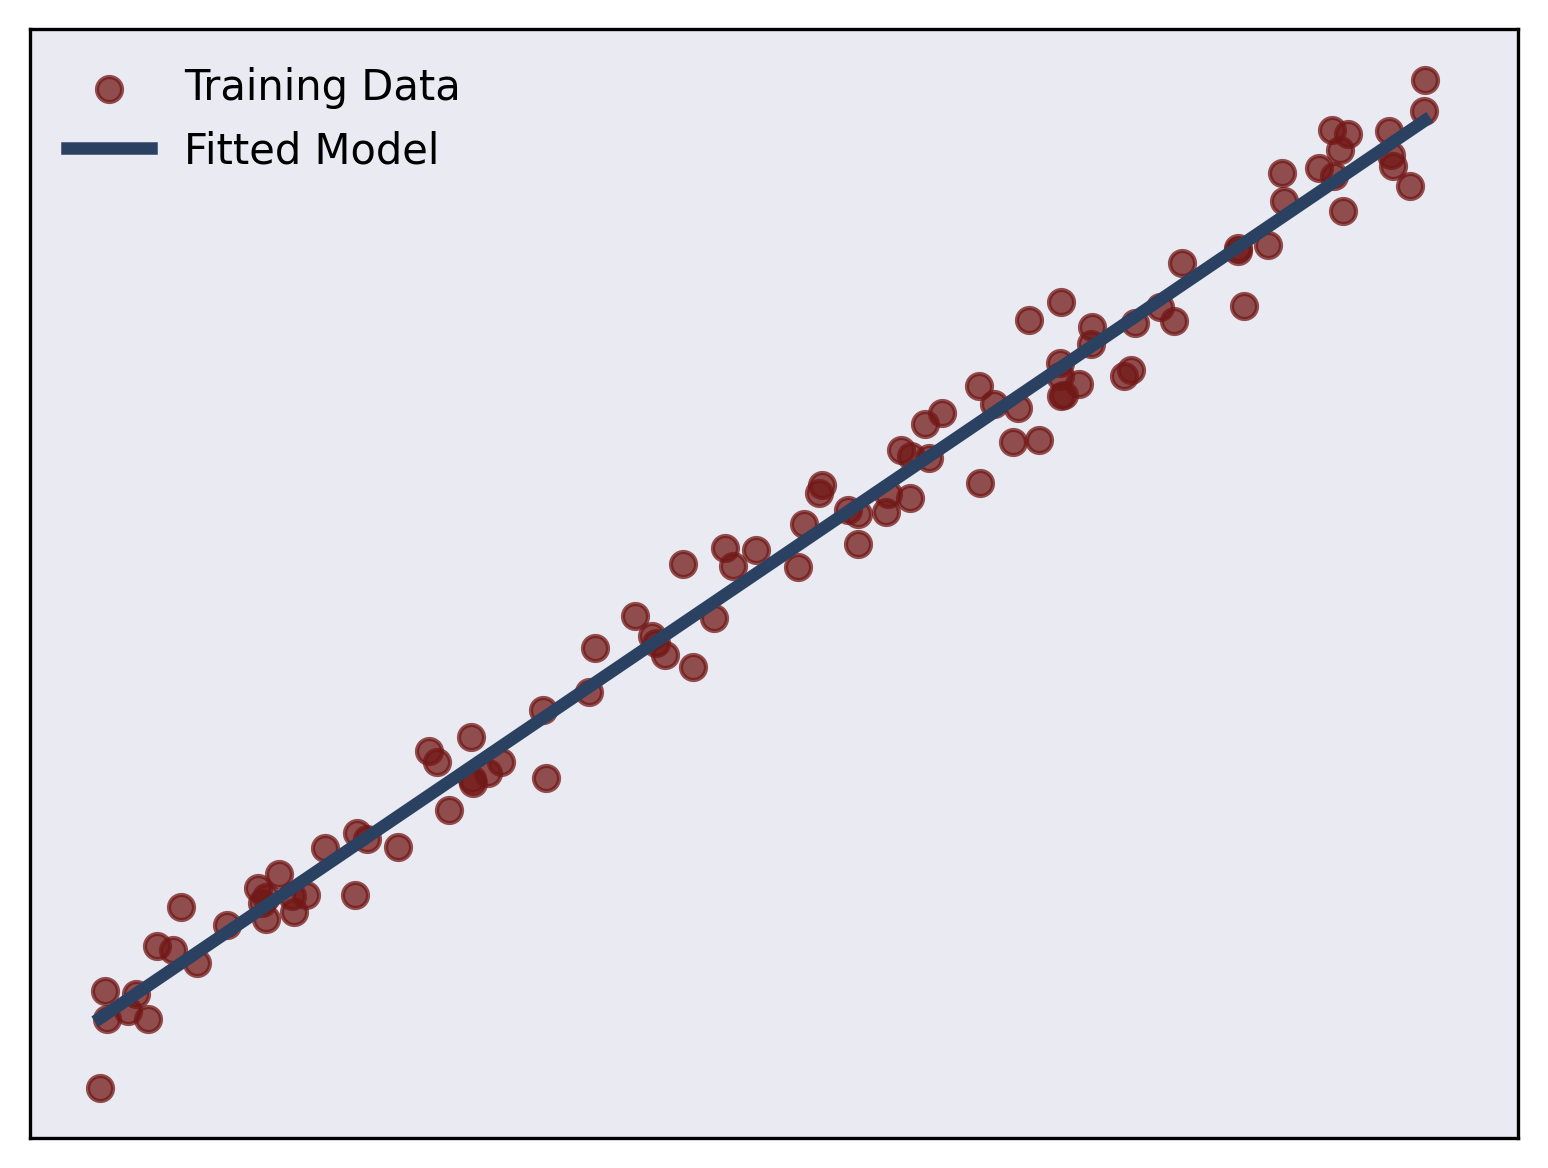
\includegraphics[width=0.45\textwidth]{source_code/goodfit_linear_model.png}
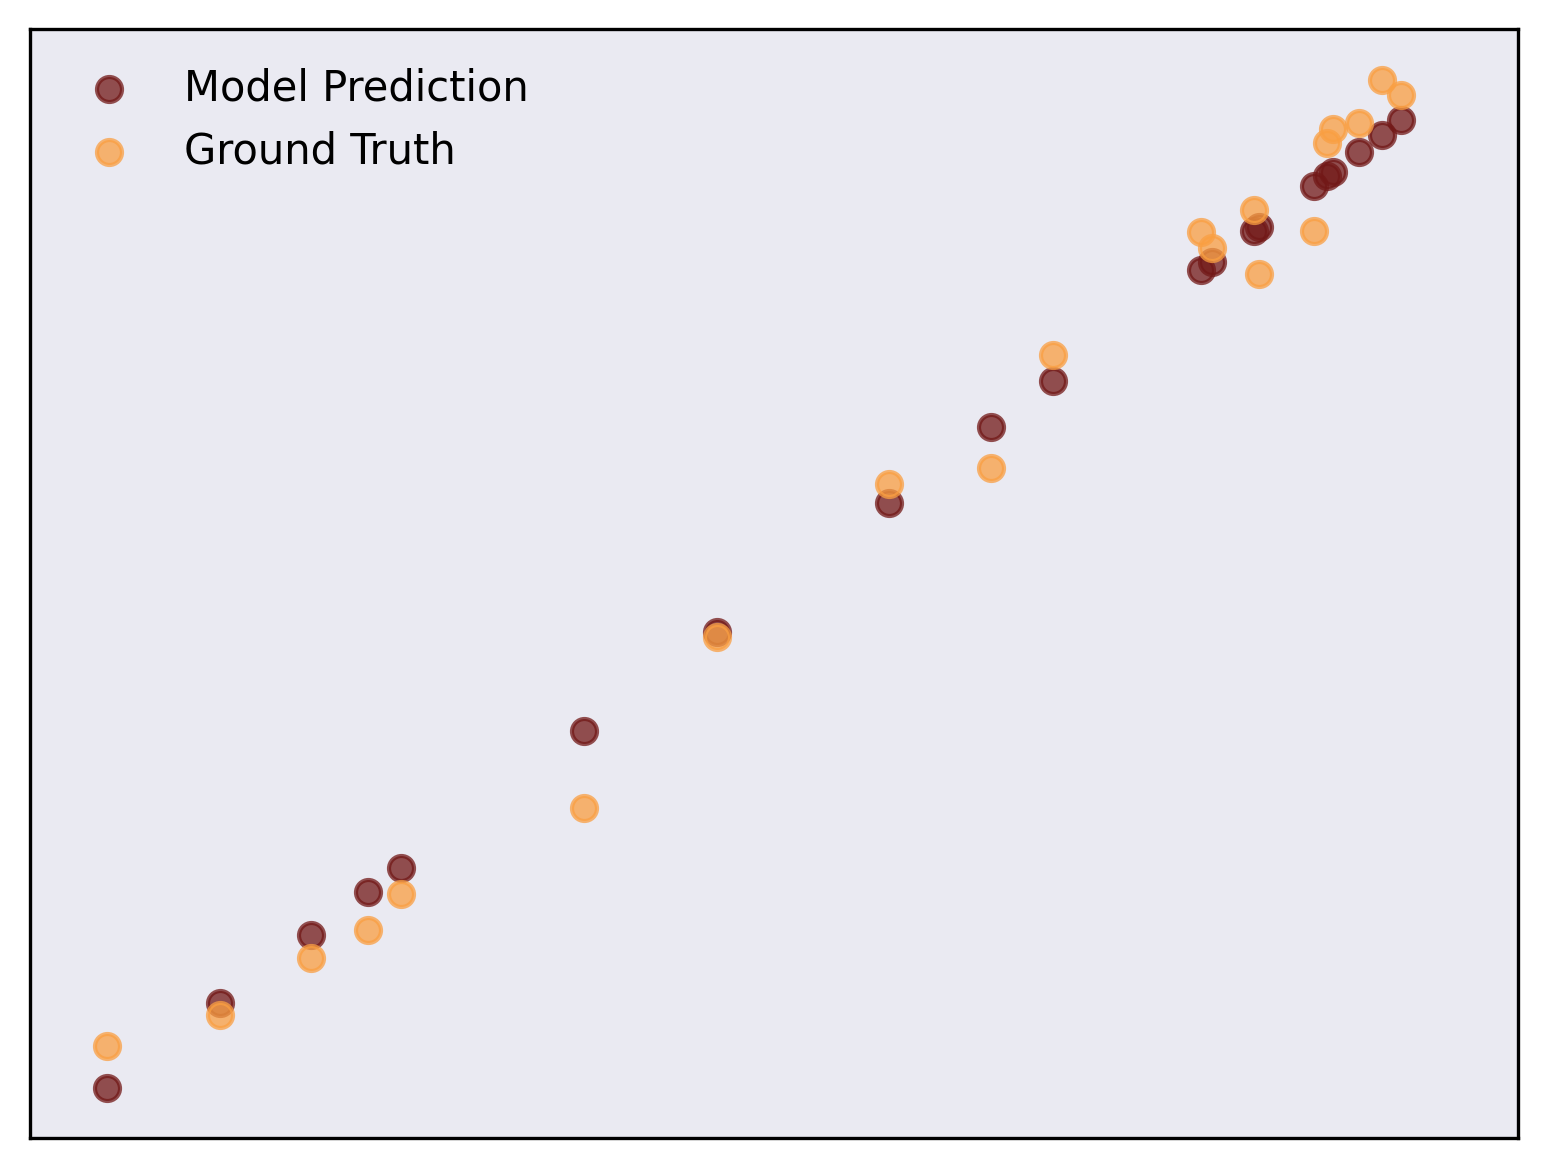
\includegraphics[width=0.45\textwidth]{source_code/goodfit_linear_testdata.png}

\end{enumerate}

I needed the following time to complete the task:

\subsection{Linear Regression: Underfit (5 points)}

Now repeat the process (load the file, fit, visualize, calculate r2\_score) with the files \texttt{non\_linear\_dataset\_100.csv} and \texttt{non\_linear\_dataset\_test.csv}.

\begin{enumerate}

\item[a)] Is the fit good or not? Why is that? 
\begin{itemize}
	\item The fit is not good because the data is not linear and the model is linear. The model can't fit the data well. (Underfit)
\end{itemize}

\item[b)] Now calculate the r\_2 score to determine the fit quantitatively. Argue how you could determine a cut-off value to determine whether a linear model is sufficient or not.
\begin{itemize}
	\item r2 score of 0.5 indicates medium correlation, r2 score of 0.7 indicates strong correlation. You could use these values as a cut-off value.
	\item another way would be to compare a linear and non-linear model and see which one fits the test data better.
\end{itemize}


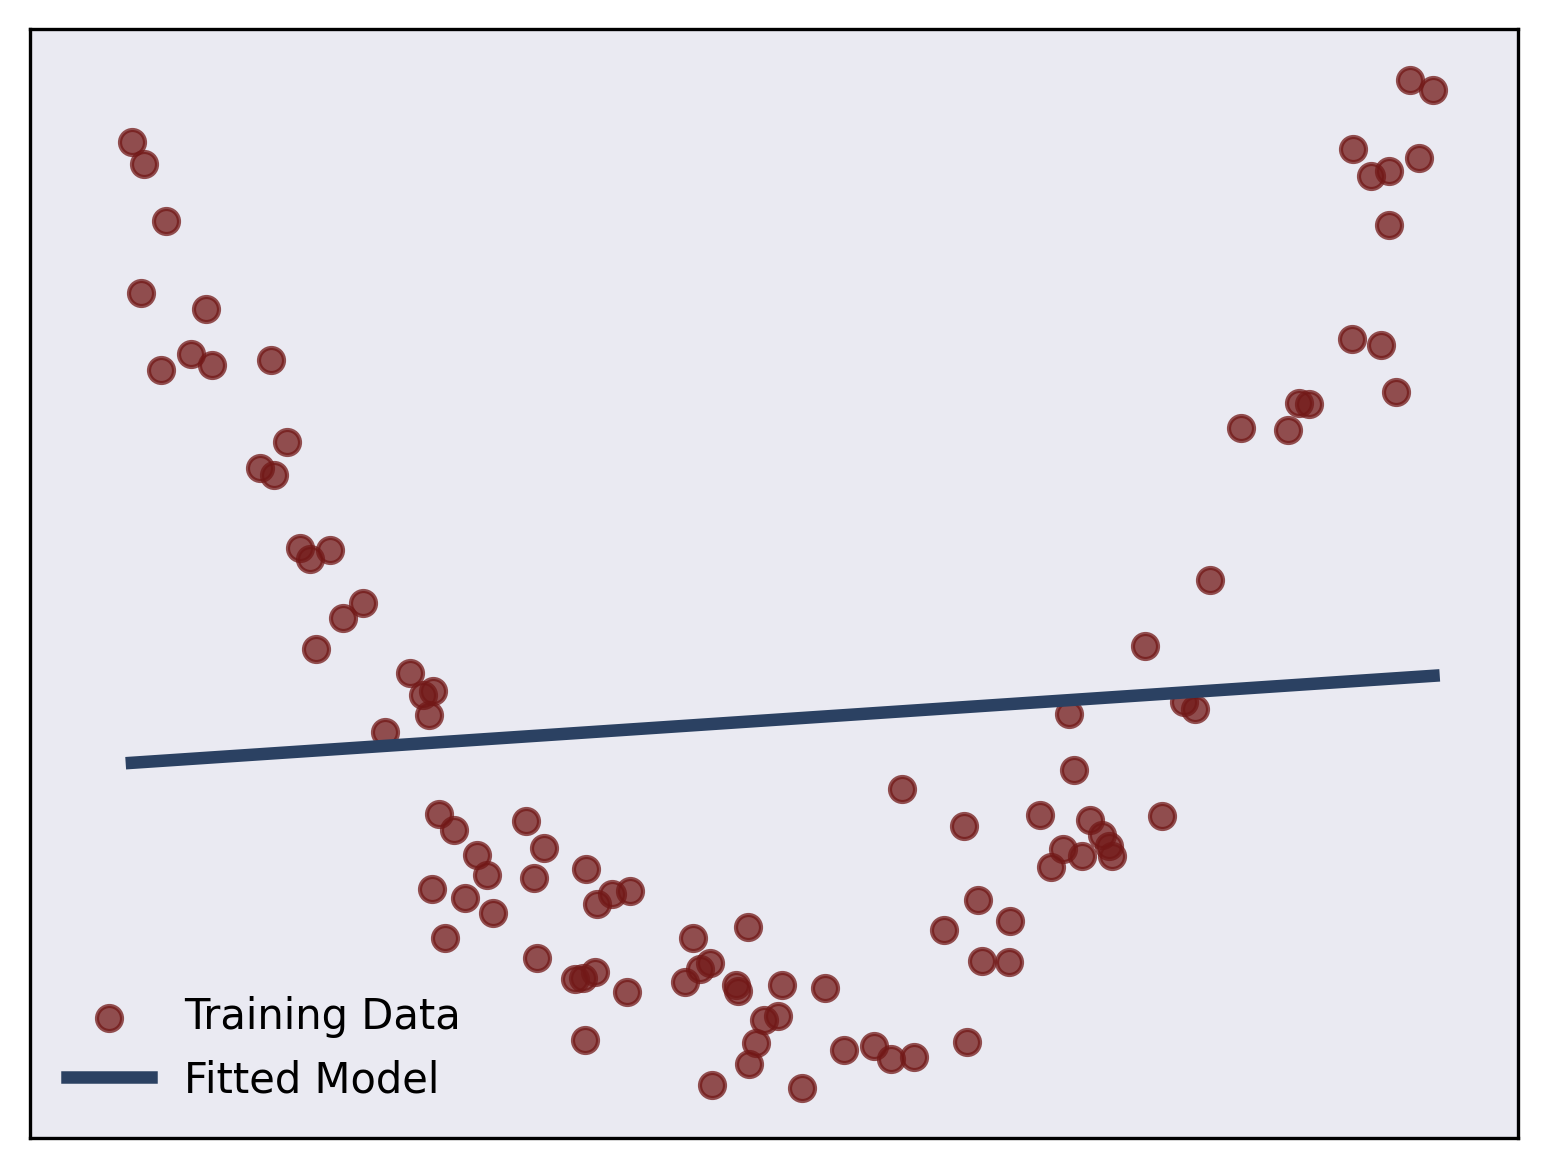
\includegraphics[width=0.45\textwidth]{source_code/underfit_linear_model.png}
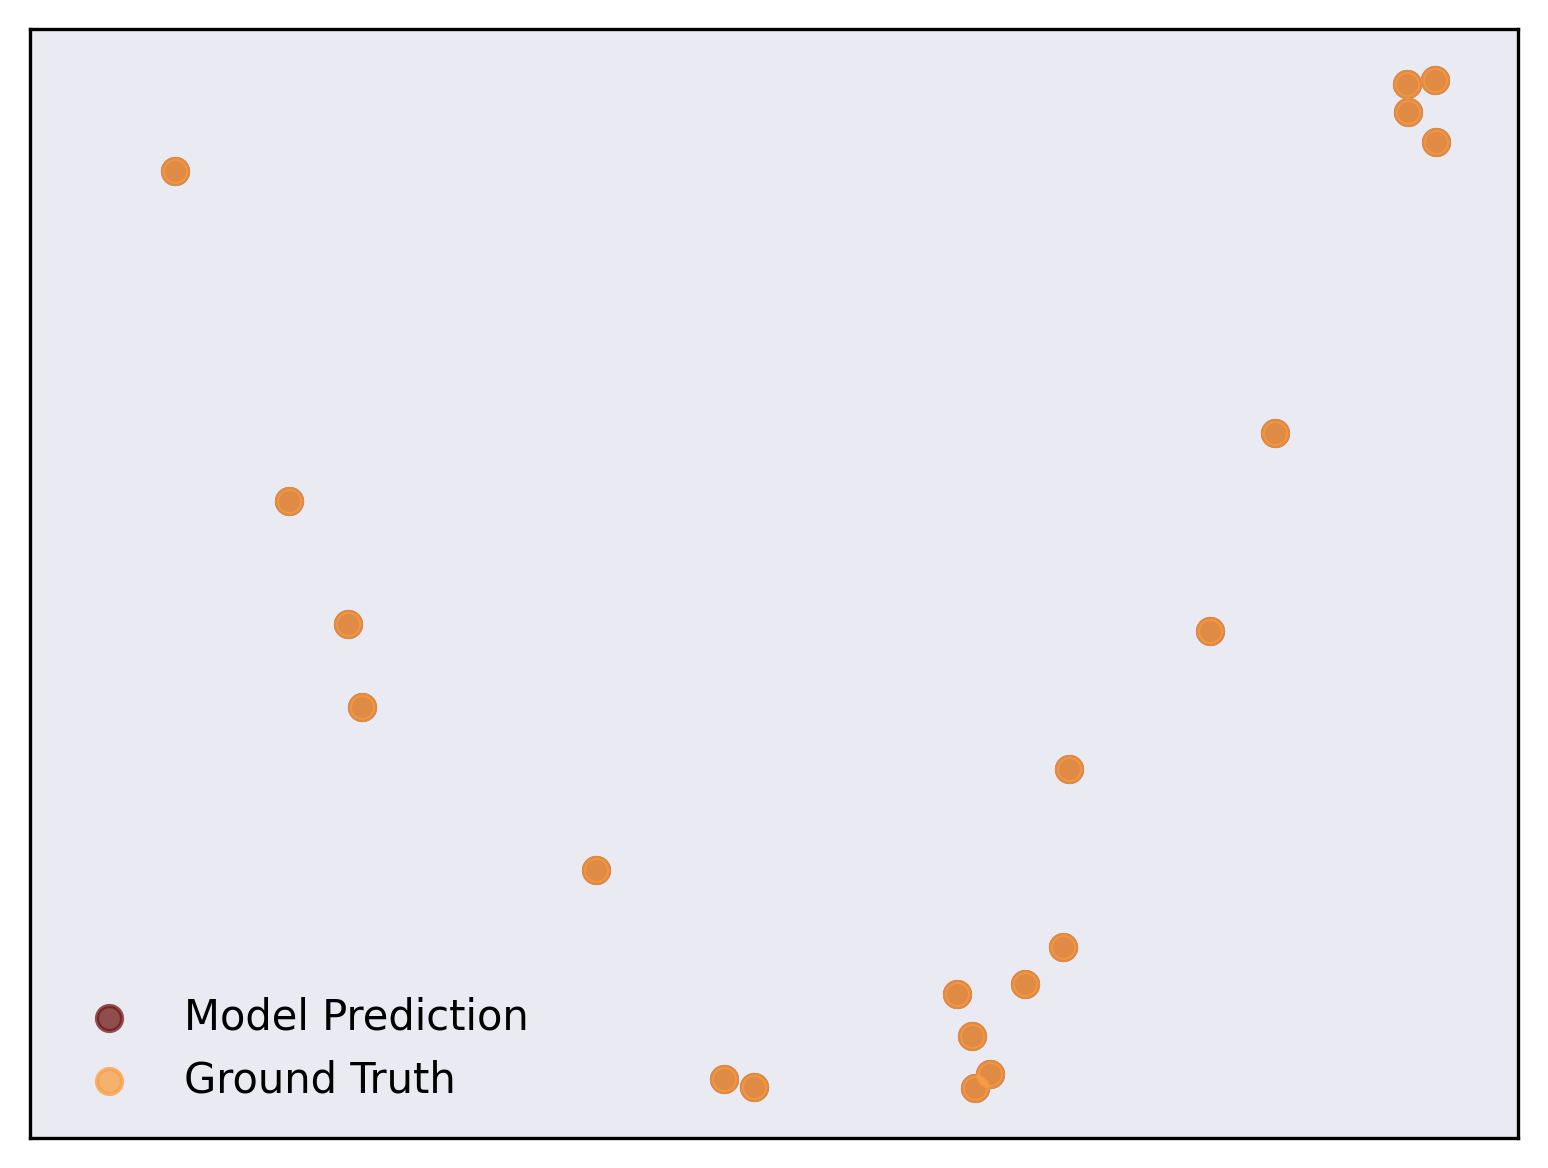
\includegraphics[width=0.45\textwidth]{source_code/underfit_linear_testdata.png}

\end{enumerate}

Recompile the latex to display the results.

I needed the following time to complete the task:

\subsection{Polynomial Regression: Fit (10 points)}

Now we use a polynomial model. This means that we increase our data by polynomial features (here: 2nd degree) and then carry out a linear regression on the
polynomial features. To do this, repeat the process (load the file, fit, visualize, calculate r2\_score) with the files \texttt{non\_linear\_dataset\_100.csv} and \texttt{non\_linear\_dataset\_test.csv}.
Use the PolynomialFeatures class from sklearn.preprocessing to create polynomial features. 

\begin{enumerate}

\item[a)] Is the fit good or not? Why?
\begin{itemize}
	\item Good fit, because high r2 score. Model capacity now sufficent for data.
\end{itemize}

\item[b)] Now calculate the r\_2 score to determine the fit quantitatively. Argue how you could determine a cut-off value to determine whether a linear model is sufficient or not.
\begin{itemize}
	\item see answer before
\end{itemize}

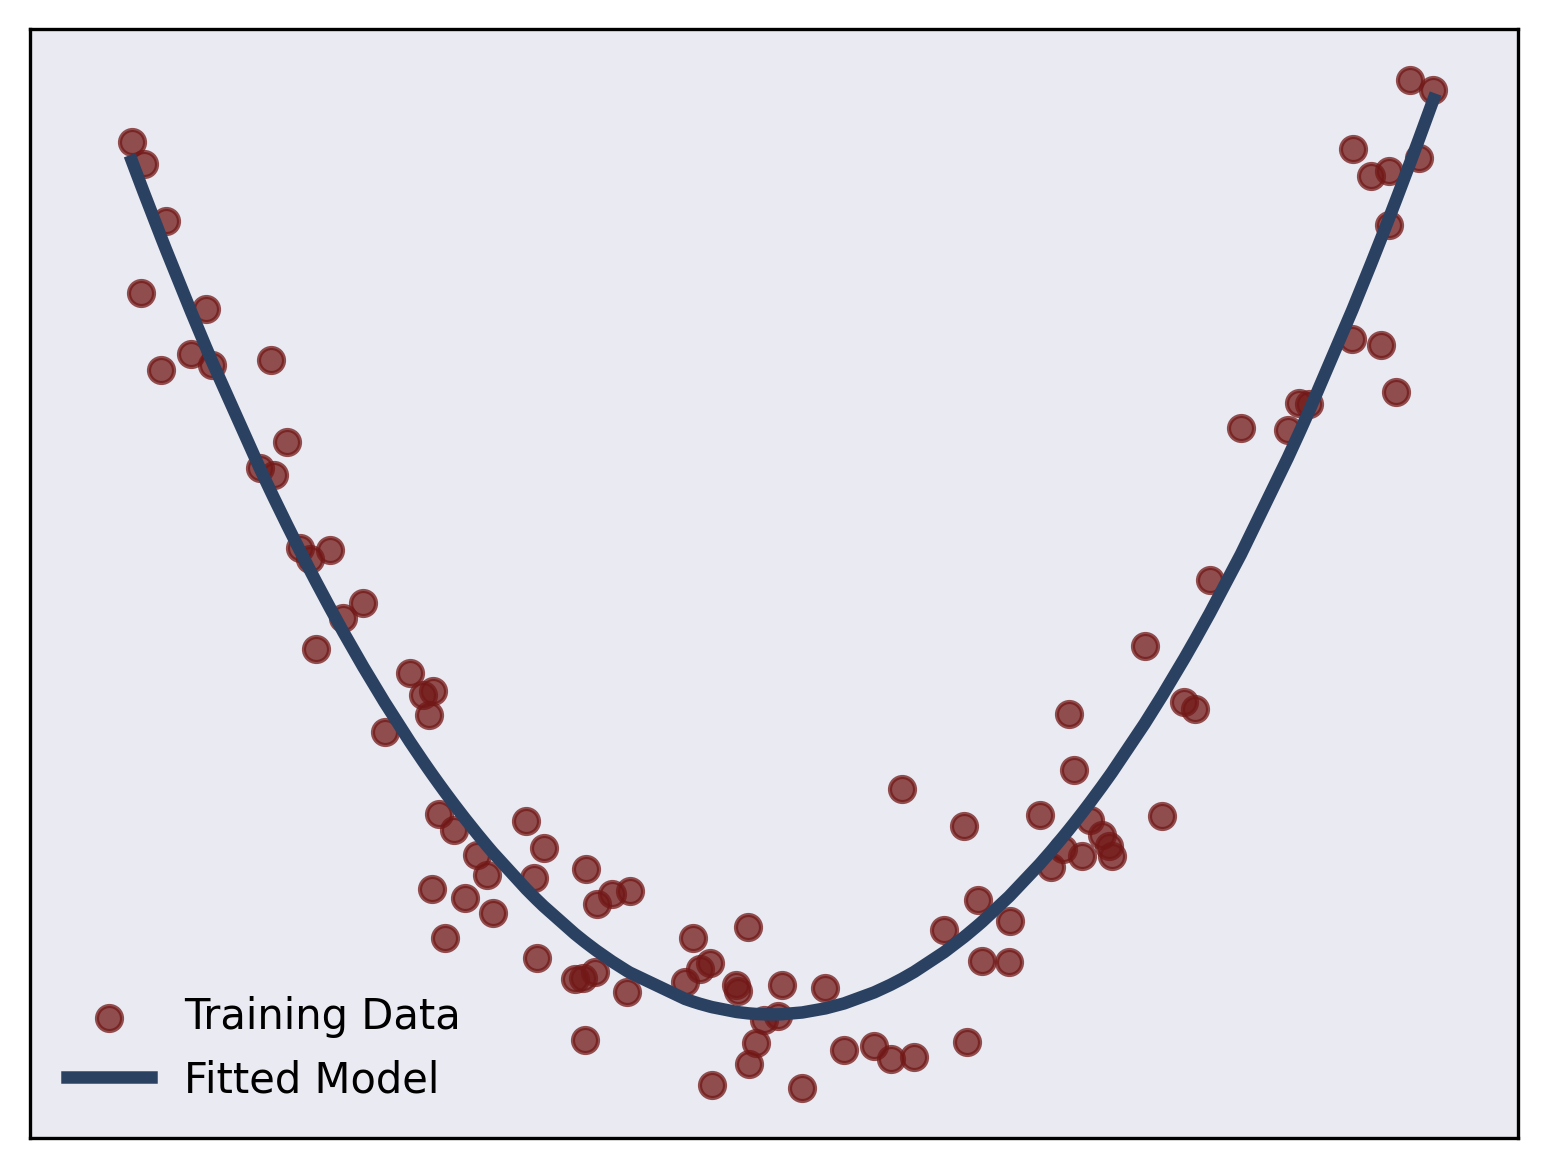
\includegraphics[width=0.45\textwidth]{source_code/goodfit_polynomial_model.png}
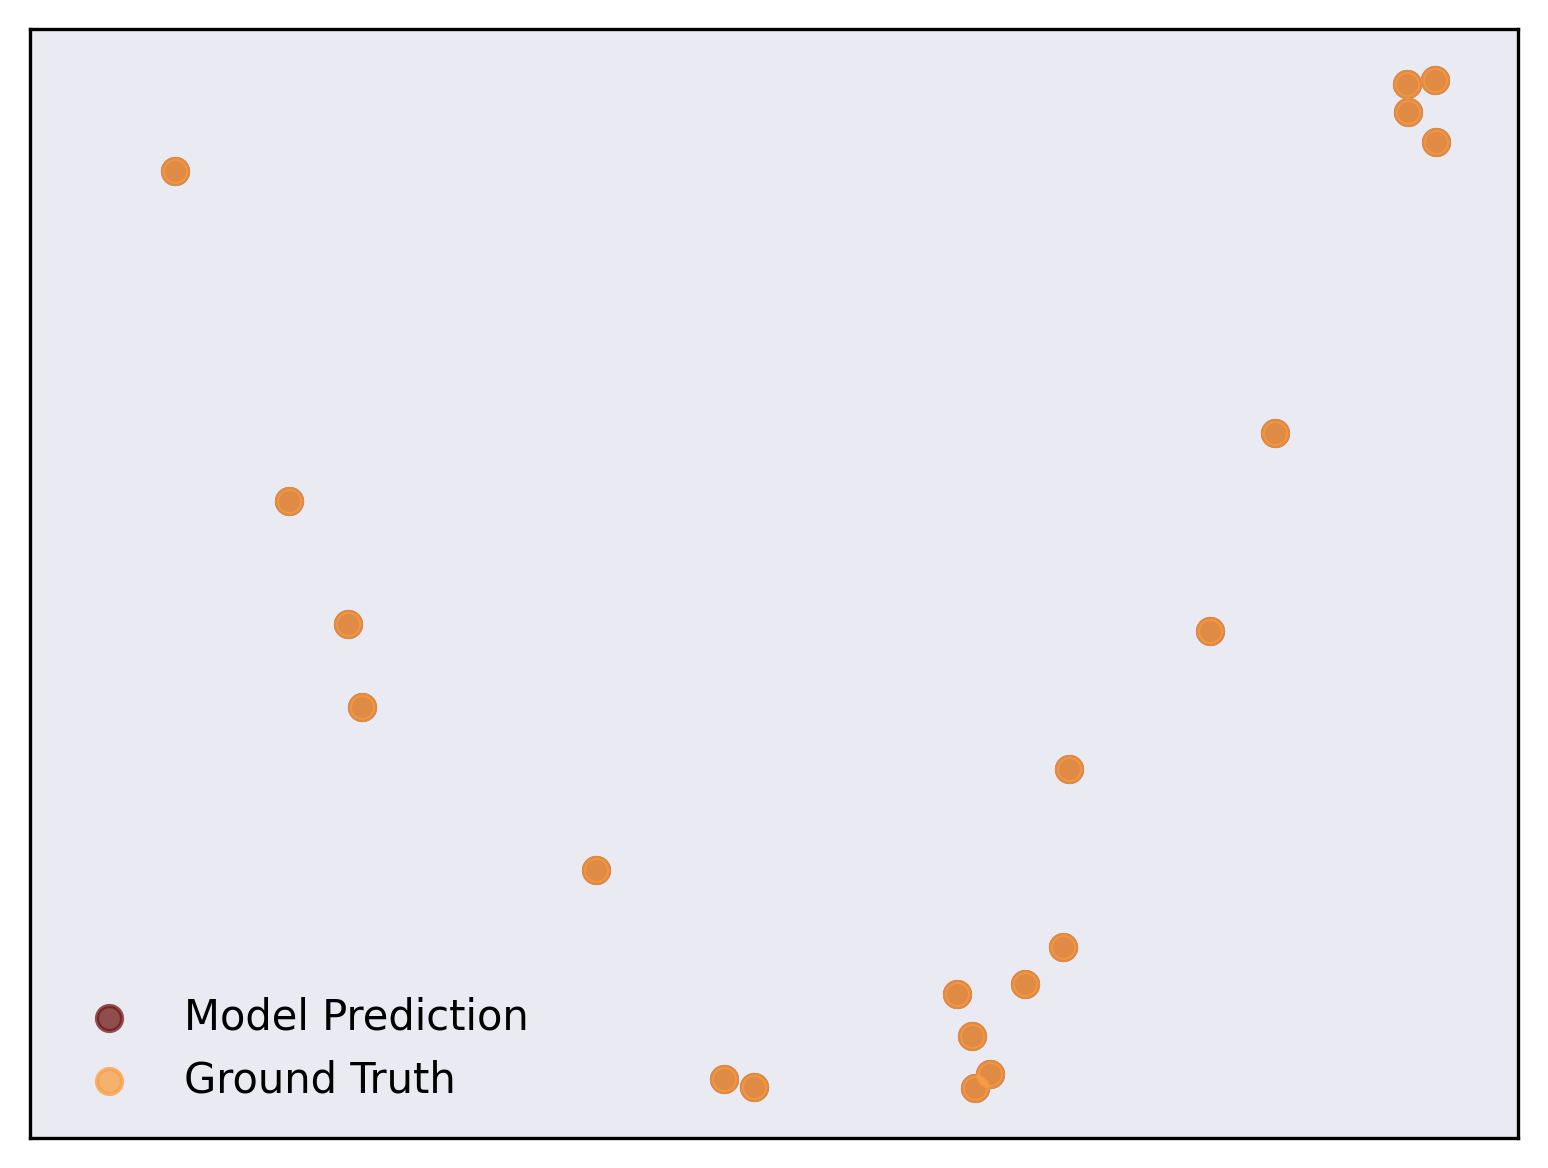
\includegraphics[width=0.45\textwidth]{source_code/goodfit_polynomial_testdata.png}

\end{enumerate}

Recompile the latex to display the results.

I needed the following time to complete the task:

\subsection{Piecewise Polynomial Regression: Overfit (10 points)}

Now we use a spline model (piecewise polynomial). To do this, we construct a spline object (degree 2) using the sklearn function make\_interp\_spline and use this to predict the test data.

\begin{enumerate}

\item[a)] Implement the regression.

\item[b)] Is the fit good or not? Why?
\begin{itemize}
	\item The fit is not good because the model is overfitting the data. The model is too complex for the data.
\end{itemize} 

\item[c)] Now calculate the r\_2 score to determine the fit quantitatively.
\begin{itemize}
	\item the r2 score is ok, its sometimes difficult to detect overfitting via the r2 score.
\end{itemize}

\item[d)] How does the fit change if you use splines of higher degree (3 or 5)? Does the result get better or worse? Why?
\begin{itemize}
	\item The fit gets worse because the model is overfitting the data more. The model is too complex for the data.
\end{itemize}

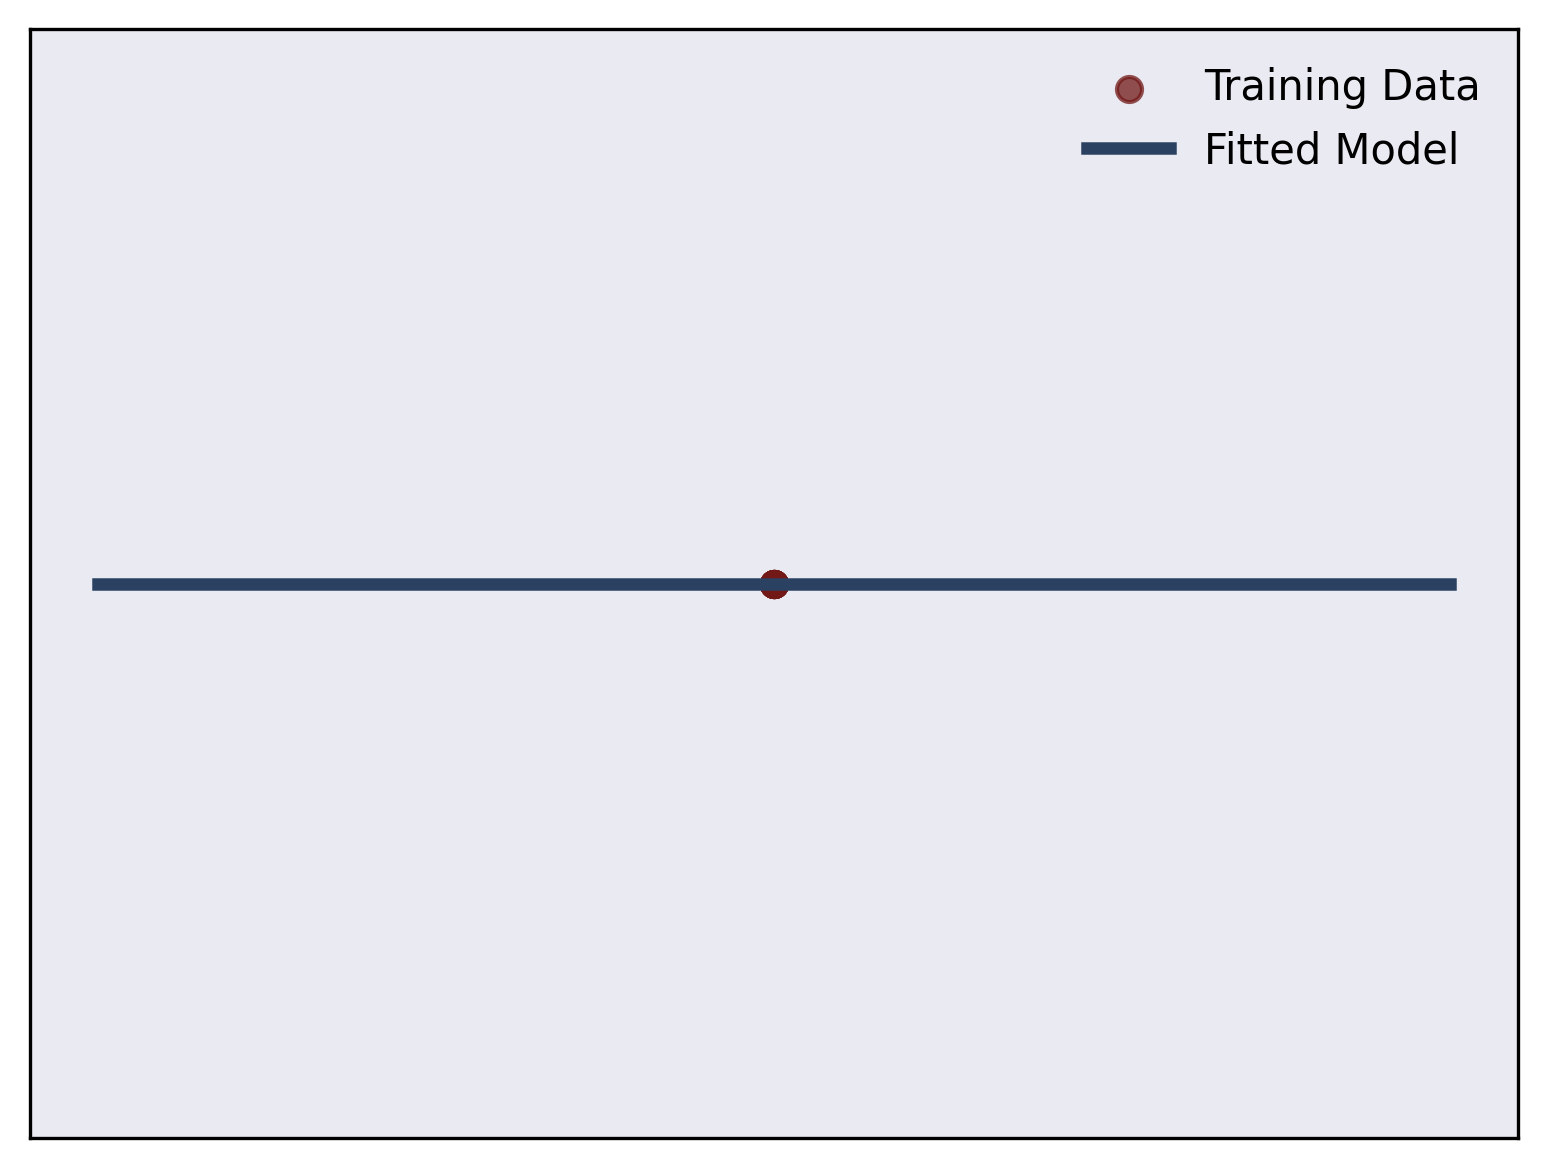
\includegraphics[width=0.45\textwidth]{source_code/overfit_spline_model.png}
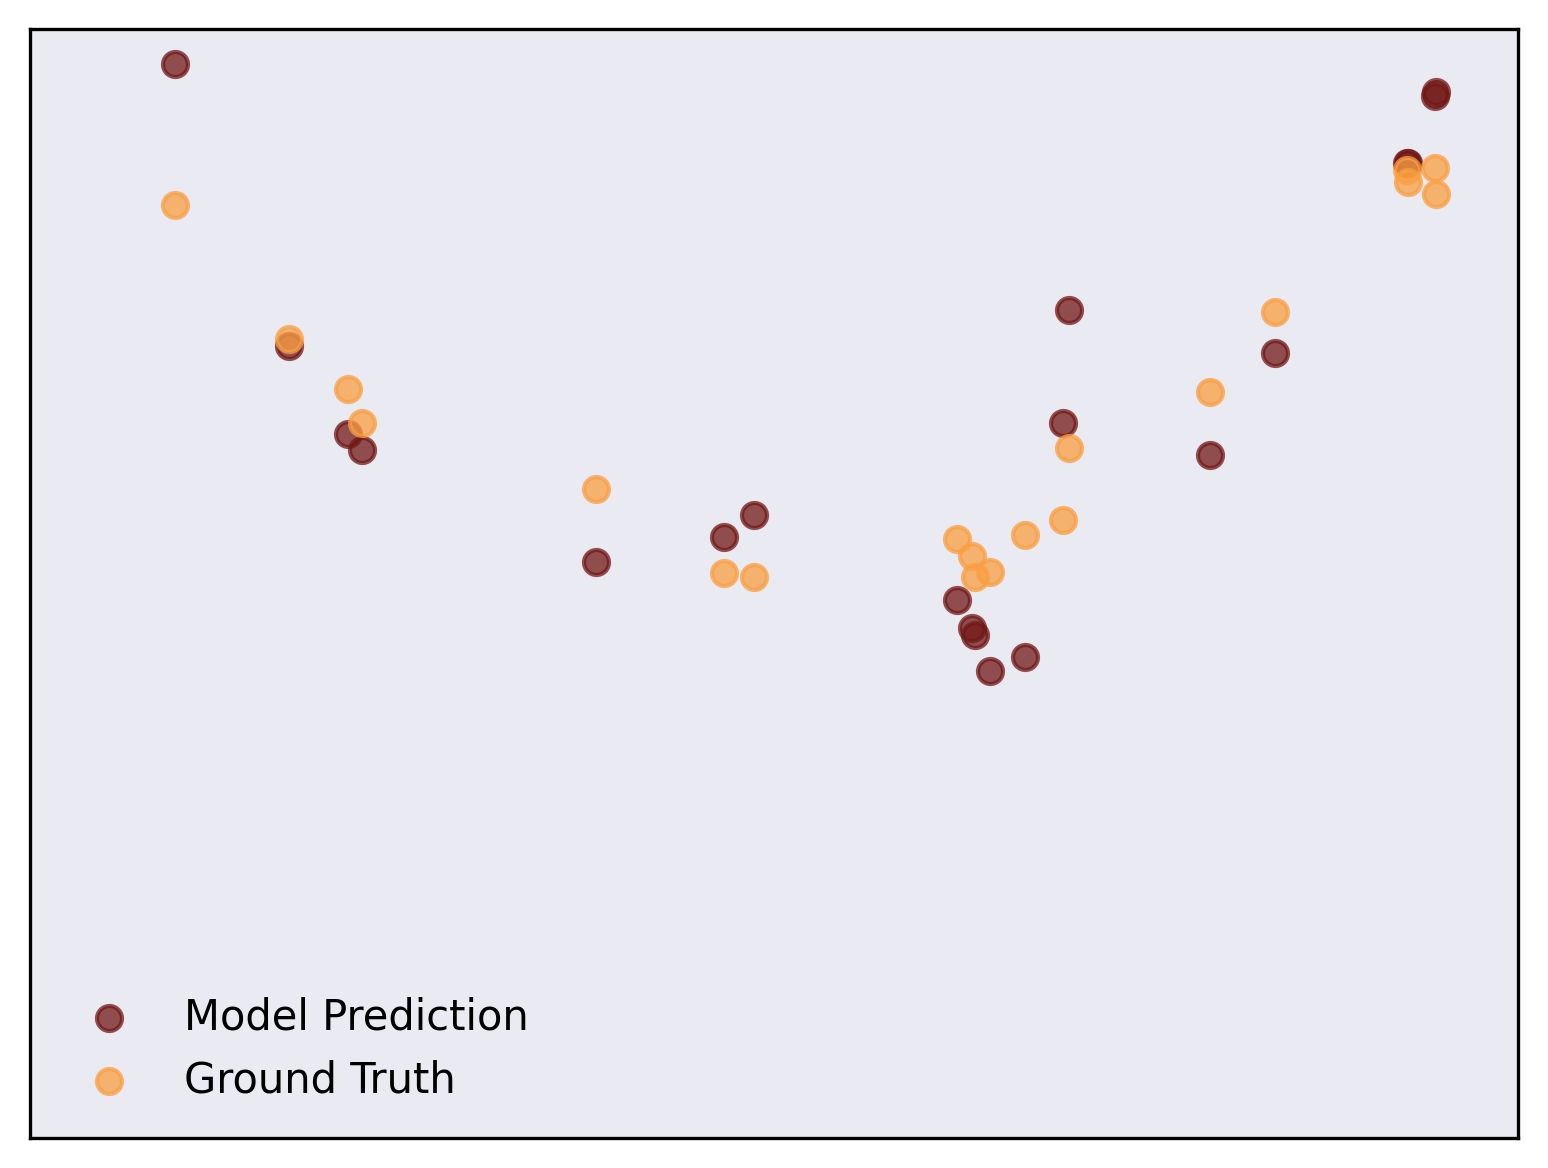
\includegraphics[width=0.45\textwidth]{source_code/overfit_spline_testdata.png}

\end{enumerate}

Recompile the latex to display the results.

I needed the following time to complete the task:

\end{document}